\documentclass{sig-alternate}

\usepackage{amssymb}
\usepackage{amsmath}
\usepackage{graphicx}
\usepackage{epsfig}
\usepackage{subfigure}
\usepackage{listings}
\usepackage{natbib}
\setlength{\bibsep}{0.0pt}
\usepackage{verbatim}
\usepackage[T1]{fontenc} 
\usepackage[hyphens]{url}
\lstset{language=ml}
\lstset{commentstyle=\textit}
\lstset{mathescape=true}
\lstset{backgroundcolor=,rulecolor=}
\lstset{frame=single}
\lstset{breaklines=true}
\lstset{basicstyle=\scriptsize\ttfamily}

\pdfpagewidth=8.5in
\pdfpageheight=11in

\begin{document}

\title{A compilation technique to increase X3D performance and safety}

\numberofauthors{4}
\author{
Giuseppe Maggiore \and Fabio Pittarello \and Michele Bugliesi \and Mohamed Abbadi\\
       \affaddr{Universit\`a Ca' Foscari Venezia}\\
       \affaddr{Dipartimento di Scienze Ambientali,}\\
       \affaddr{Informatica e Statistica}\\
       \email{\{maggiore,pitt,michele,mabbadi\}@dais.unive.it}
}

\date{}

\maketitle

\begin{abstract}
As virtual worlds grow more and more complex, virtual reality browsers and engines face growing challenges. These challenges are centered on performance on one hand (an interactive framerate is always required) and complexity on the other hand (the larger and more articulated a virtual world, the more immersive the experience).

The usual implementation of an engine or browser for running virtual worlds features an object-oriented architecture of classes. This architecture is a source of often underestimated overhead in terms of dynamic dispatching, and dynamic lookups by scripts when they try to access portions of the scene are both costly and possible sources of mistakes.

In this paper we discuss how we have tackled the problem of increasing performance in X3D browsers while also making scripts safe. We have used a compilation technique that removes some overhead and which allows us to introduce safety for scripts that access the state
\end{abstract}

\category{D.1.1}{Programming Techniques}{Applicative (Functional) Programming} 
\category{D.2.2}{Soft\-ware Engineering}{Software Libraries}[Design Tools and Techniques]
\category{D.2.13}{Soft\-ware Engineering}{Reusable Software}[Domain engineering, Reusable libraries, Reuse models]
\category{D.3.3}{Programming Languages}{Language Constructs and Features}
\category{D.3.4}{Pro\-gramming Languages}{Processors}[Optimization, Run-time environments]
\category{H.5.1}{Information Systems}{Information Interfaces and Presentation}[Multimedia Information Systems]

\terms{Performance,Reliability,Languages}

\keywords{x3d, performance, safety, compilation}

\section{Introduction}
\label{sec:intro}
%%%%%%%%%%%%%%%%%%%%%%%%%%%%%%%%%%%%%%%%%%%%%%%%%%%%%%%%%%
% intro.tex
%%%%%%%%%%%%%%%%%%%%%%%%%%%%%%%%%%%%%%%%%%%%%%%%%%%%%%%%%%


\begin{figure}
\begin{center}
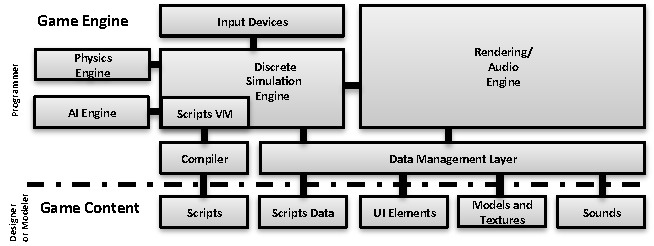
\includegraphics[scale=0.8]{engine_architecture.pdf}
\end{center}
\label{fig:data_driven_games}
\caption{Data-driven engine architecture, from \cite{SGL}}
\end{figure}

Virtual reality browsers face big challenges centered on performance and complexity. Performance is needed because the framerate at which the virtual world is rendered and animated must be high enough to give the user a feeling of smoothness. The scene must be rendered at least at 30 frames per seconds, but higher framerates (e.g. 60 frames per second) are perceived by the user as more pleasant.

Both the visual and logical complexities of a virtual world are very important. Visual richness gives the user the impression of a more realistic and detailed world, with many beautifully rendered objects, while logical complexity permits articulated responses that give the user the feeling of being part of a realistic world with its own set of rules and internal laws.

One of the most important tasks for developers of interactive worlds is to find the right trade-off between these sometimes conflicting requirements. Increasing performance requires a mixture of compromise (reducing the size of the world or ``dumbing down'' its responses) and time-consuming low-level optimization. We believe that automated optimization of interactive applications is a fundamental frontier if we wish to enable developers to build richer worlds without exponentially increasing costs.

Modern 3D browsers and engines are based on a data-driven architecture as shown in Figure \ref{fig:data_driven_games}, taken from \cite{SGL}.

In a data-driven engine the engine contains only general knowledge about virtual worlds, but nothing specific about the peculiar features of a specific virtual world. The specific virtual world will be loaded from the game content in the form of configuration files and scripts. A data-driven engine loads from files two main datasets:

\begin{itemize}
\addtolength{\itemsep}{-0.5\baselineskip}
\item a \textbf{scene}, the set of entities that populate the virtual world
\item \textbf{scripts}, the set of (possibly complex) behaviors that animate the scene entities
\end{itemize}

The scene is composed by a heterogeneous set of entities, each of a different kind. Entities may be virtual characters, trees, 2d or 3d models; entities may also be purely logical and invisible entities such as timers, triggers and proximity sensors.

Scripts give depth to a scene by implementing complex interrelationships between entities. Scripting can be done at three different levels of increasing complexity and expressive power:

\begin{itemize}
\addtolength{\itemsep}{-0.5\baselineskip}
\item \textit{routing} is a simple transmission of values from one entity to another
\item more complex scripts can perform data conversions when moving information between entities
\item even more advanced scripts can create, remove or modify entities of a scene
\end{itemize}

The usual implementation of an engine (see \cite{GAME_OO_HIERARCHY}) features an object-oriented architecture of classes. At the root of this architecture is a class that represents the most generic entity, and from which all other entities are derived. The engine maintains a list of these generic entities, which are all updated and handled through a set of virtual functions. This architecture is a source of often underestimated overhead. Dynamic dispatching is not too costly for a few calls, but when we have many entities, the cost of invoking various virtual functions many times for each frame can become very high. Sometimes the cost of the dynamic dispatching architecture may become higher than the cost of the actual operations being dispatched.

Scripts usually access the scene dynamically. This means that a script must look for the right entities with a mixture of lookups by name and unsafe casts. For example, consider how a Java script may access the \texttt{time} field of a \texttt{myClock} node of type \texttt{timer}:

\begin{lstlisting}
\addtolength{\itemsep}{-0.5\baselineskip}
X3DNode myClock = 
 mainScene.getNamedNode("myClock");
SFTime time = 
  (SFTime) myClock.getField("time");
\end{lstlisting}

This style is unsafe, since \texttt{myClock} may not exist or it may have the wrong type, and it also incurs in significant overhead.

In this paper we will focus exclusively on the X3D language, since it is a recognized standard and it offers a good benchmark to test virtual worlds where we can specify our scene and its various scripts. In the paper we show how we have tackled the problem of increasing performance in X3D browsers while also making scripts safe. We have used a simple compilation technique that removes many unnecessary dynamically dispatched invocations; this technique also allows us to introduce safety for scripts that access the state, so that they do not need to perform unsafe dynamic lookups when searching for specific nodes. To the best of our knowledge, this is the first approach that experiments with compiling X3D scripts and scenes in order to achieve greater performance and safe scripts. None of the previous approaches we are aware of focuses on compilation of X3D as a means to achieve both higher performance (by reducing overhead) and safety (by introducing compile-time checks). Higher performance through compilation includes a long list of research work such as \cite{OPT1,OPT2,OPT3} which has shown that compilation can yield better runtime performance by reducing dynamic overhead and improving other properties of the generated code. Similarly, introducing safety in dynamic languages such as scripting systems has been studied in general in the context of generating typed programs from untyped scripts in \cite{SAFESCRIPTS1}, and the problem of statically typing information which is generally untyped has also been explored in the Haskell community in \cite{SAFESCRIPTS2} among many others.

In Section \ref{sec:solution_workflow} we discuss the general architecture of our system. In Section \ref{sec:compiling_scene} we show how our technique generates the code and the type definitions that represent a scene. In Section \ref{sec:case_study} we show an example of a compiled scene and its routes. In Section \ref{sec:benchmarks} we report some benchmarks that show speed increasing when rendering a sample scene with just nodes and routes by applying our technique. Finally, in Section \ref{sec:compiling_scripts} we discuss how we represent scripts that externally access the scene.

 

\section{Solution Workflow}
\label{sec:solution_workflow}
%%%%%%%%%%%%%%%%%%%%%%%%%%%%%%%%%%%%%%%%%%%%%%%%%%%%%%%%%%
% solution_workflow.tex
%%%%%%%%%%%%%%%%%%%%%%%%%%%%%%%%%%%%%%%%%%%%%%%%%%%%%%%%%%

\begin{figure}
\begin{center}
\includegraphics[scale=0.6]{Solution_workflow.png}
\end{center}
\label{fig:solution_workflow}
\caption{Solution workflow}
\end{figure}

In Figure \ref{fig:solution_workflow} we can see a diagram depicting the steps used by our system when processing an X3D scene (plus its accompanying scripts). In the figure red blocks represent data while the blue blocks represent computations.
We start with an X3D file which describes our scene. This file may contain some scripts as routes, in \texttt{script} node, or the scripts may be stored into an external file. There are two layers of transformations described by our system:

\begin{itemize}
\addtolength{\itemsep}{-0.5\baselineskip}
\item a transformation from the original external scripts into our F\# scripts
\item a transformation from the original entities and routes of the X3D file into the final program
\end{itemize}

In the current development stage we have implemented part of the first transformation (we translate those scripts that are expressed as routes) and the second transformation (we can process any scene entity). The X3D scene and its routes are translated into F\# source code. This source code contains a type definition that describes the entire scene and the routes, plus an update function that translates the activation of scripts as a consequence of the changes in the entities that result from a user action or from the temporal evolution of the scene. Such conversion therefor supports the translation of regular X3D nodes that describe shapes and the various scene entities, and also routing nodes that describe basic scripts.

Our system supports \textit{external scripts}, that is any script that is not expressed as a route, but only if they are provided already translated to F\#; this means that our system cannot translate and process scripts written in Javascript and Java, but it can process those scripts if the translation has been done by hand. External scripts in F\# are validated against our type definitions, to ensure that they correctly access the scene. If their validation succeeeds, the final program is produced that integrates both the scene and all the scripts. This second processing gives our system support for any other scripts which are not easily expressed with routes.

We have used F\# \cite{FRIENDLY_FSHARP,FSHARP}, a multi-paradigm functional programming language targeting the .NET Framework. It is a variant of ML and is largely compatible with the OCaml implementation. F\# enjoys full support in the .NET Framework, meaning that it can take advantage of all .Net libraries (such as XNA for game development, which is most useful to us) and powerful IDEs such as Visual Studio and MonoDevelop.

\section{Compiling The Scene}
\label{sec:compiling_scene}
%%%%%%%%%%%%%%%%%%%%%%%%%%%%%%%%%%%%%%%%%%%%%%%%%%%%%%%%%%
% compiling_scene.tex
%%%%%%%%%%%%%%%%%%%%%%%%%%%%%%%%%%%%%%%%%%%%%%%%%%%%%%%%%%

In this section we show an outline of our compilation technique. 

The first step our compiler performs is deserializing the xml definition of our X3D scene. The scene is then processed and turned into a record, a type definition that describeds the static structure of our scene. The record contains:

\begin{itemize}
\addtolength{\itemsep}{-0.5\baselineskip}
\item a field for each static node of the scene; each field has the name of the node if the node has a \texttt{DEF} attribute
\item a field for a list of dynamic nodes
\item a field for a list of active scripts
\end{itemize}

A sample state for a scene with a timer and a box could be:

\begin{lstlisting}
type Scene  =
  {
    myClock       : Timer 
    box           : Box
    dynamic_nodes : List<Node>
    script        : Script
  }
\end{lstlisting}

Where \texttt{Timer} and \texttt{Box} are the concrete classes for a timer and a box respectively, and they both inherit from the \texttt{Node} class.
A list of nodes is needed to represent the dynamic portions of the scene, and a list of scripts maintains the sequence of currently running scripts.

This state definition is quite important, since it represents the interface between our scene and our scripts, and since it allows us fast lookups of specific nodes. Finding a node now just requires reading from a field in the state, an operation which is both fast and certain not to fail. For example, looking for the \texttt{time} field of the \texttt{"myClock"} node would simply require writing:

\begin{lstlisting}
scene.myClock.time
\end{lstlisting}

We then proceed to the initialization of the state. This amounts to creating instances of each node, and then assigning these instances to the fields of the \texttt{scene} variable.

An \texttt{update} function is then constructed that performs the update of all the statically known fields of the state, and which also executes the various routes of the scene. Also, the \texttt{update} function invokes the (dynamically dispatched) \texttt{update} function of each dynamic node; this is necessary because it would be unrealistic to hope that a complex virtual world can exclusively rely on statically known nodes, and a balance must be struck between optimizing static nodes and supporting dynamic ones.

The \texttt{update} function also performs a tick for all currently running scripts.

The update function that updates the state seen above would simply become:

\begin{lstlisting}
let update (dt:float32) =
  scene.myClock.update dt
  scene.box.update dt
  for node in scene.dynamic_nodes do
    node.update dt
  scene.script.update dt
\end{lstlisting}

We could add a simple route that moves the \texttt{box} node along the Y-axis according to the current time of the \texttt{myClock} node by adding the following line of code to the \texttt{update} function:

\begin{lstlisting}
  scene.box.Position.Y <- scene.myClock.Time
\end{lstlisting}

In general, routes are simple assignments when translated into our system.

\section{A More Detailed Example}
\label{sec:case_study}
Mini Galaxy Wars.

\section{Benchmarks}
\label{sec:benchmarks}
%%%%%%%%%%%%%%%%%%%%%%%%%%%%%%%%%%%%%%%%%%%%%
% BENCHMARKS
%%%%%%%%%%%%%%%%%%%%%%%%%%%%%%%%%%%%%%%%%%%%%

- Windows, Xbox, Wp7 (, iPad?)
- memory recycling
- parallel execution
- query optimization
 

\section{External Scripts}
\label{sec:compiling_scripts}
%%%%%%%%%%%%%%%%%%%%%%%%%%%%%%%%%%%%%%%%%%%%%%%%%%%%%%%%%%
% compiling_scripts.tex
%%%%%%%%%%%%%%%%%%%%%%%%%%%%%%%%%%%%%%%%%%%%%%%%%%%%%%%%%%

Scripting is a very important part of game development \citep{BETTER_SCRIPTS_GAMES}. For this reason we have adapted to our system a scripting solution that is derived from game engines. Whereas many game engines either use Lua, Python or even C\# as scripting languages (with various advantages and disadvantages) \cite{SCRIPTING_LUA,SCRIPTING_PYTHON, UNITY_YIELD} we have used F\# which we believe offers a powerful mix of the best features of all these languages: coroutines, flexibility and a lightweight syntax make F\# scripts similar to LUA and Python while static typing and support for .Net libraries and IDEs put F\# on par with C\# in terms of broader support.

To give additional expressive power to our scene, we add support to external scripts; external scripts are all those scripts that cannot be expressed in terms of routes. External scripts are very general, that is they can perform complex data conversions when copying values across entities, and they may even create, remove and modify nodes in any way possible. To represent external scripts, rather than using arbitrary objects that can access the state we have chosen to use coroutines, a widely used mechanism for representing computations in interactive applications \cite{PYTHON_COROUTINES,GPU_GEMS_6}. Coroutines are subroutines that can be suspended and resumed at certain locations. With coroutines the code for a SM is written ``linearly'' one statement after another, but each action may suspend itself (an operation often called ``yield'') many times before completing. A coroutine stores a temporary, internal state transparently inside its continuation.

We build a monadic framework \cite{COMPR_MON,DECL_IMP,EFF_MON,MOGGI_MON} for coroutines that allows us greater customization flexibility. This way we can define our own system for combining scripts running them in parallel, concurrently, etc. For a detailed discussion of this monadic framework for scripts and coroutines see \cite{X3D_TR1}.

A script in our system is defined as a normal F\# program surrounded by \texttt{\{ \}} brackets. A script runs another script with the statements \texttt{let!} and \texttt{do!}, and scripts can be combined with a small set of operators.

The main operators to combine scripts are:
\begin{itemize}
\item \texttt{parallel} ($s_1 \wedge s_2$) executes two scripts in parallel and returns both results
\item \texttt{concurrent} ($s_1 \vee s_2$) executes two scripts concurrently and returns the result of the first to terminate
\item \texttt{guard} ($s_1 \Rightarrow s_2$) executes and returns the result of a script only when another script evaluates to \texttt{true}
\item \texttt{repeat} ($\uparrow s$) keeps executing a script over and over
\end{itemize}

A sample script that moves the box \texttt{myBox} when the user enters a certain region \texttt{myRegion} could be the following:

\begin{lstlisting}
let my_script (scene:Scene) =
  let rec animate =
    script {
      if scene.myBox.Position.Y < 100.0f then
        scene.myBox.Position.Y <- scene.myBox.Position.Y + 0.1f
        do! animate }
  script {
    do! guard
         script {
           return inside(scene.Camera.Position, myRegion) }
         animate }
\end{lstlisting}

Notice that our script has a parameter of type \texttt{Scene}. If this parameter is used incorrectly (for example the scene this script is applied to does not have a \texttt{Box} node with name \texttt{myBox}) we will get a compile-time error. This makes it easier to build larger, reusable script modules since a mistake in using a pre-made module is easier to spot and requires less testing. Using scripts which have been made for different scenes would require extensive testing to ensure at least that all node accesses are correct.

Our scripting system is expressive enough to represent many scripts running together, even if at a first glance it may appear that our system supports only a single script. By using the \texttt{parallel} operator we can combine together a large number of scripts. For example, let us say we have many scripts $s_1, ... , s_n$ that must all run together with our scene. Each scripts has a different duration, that is the not all scripts will end at the same time (indeed, a script may even run indefinitely). The main script would chain each of the various actual scripts in the following manner:

\begin{lstlisting}
let my_script (scene:Scene) =
  parallel $s_1$ (parallel $s_2$ ... $s_n$) ... )
\end{lstlisting}
 

\section{Conclusions and future work}
\label{sec:conclusions}
%%%%%%%%%%%%%%%%%%%%%%%%%%%%%%%%%%%%%%%%%%%%%%%%%%%%%%%%%%
% conclusions.tex
%%%%%%%%%%%%%%%%%%%%%%%%%%%%%%%%%%%%%%%%%%%%%%%%%%%%%%%%%%

Scripts are an important and pervasive aspect of computer games. Scripts simplify the interaction with computer game engines to the point that a designer or an end-user can easily customize gameplay. Scripting languages must support coroutines because these are a very recurring pattern when creating gameplay modules. Scripts should be fast at runtime because games need to run at interactive framerates. Finally, the scripting runtime should be as modular and as programmable as possible to facilitate its integration in an existing game engine.

In this paper we have shown how to use meta-programming facilities (in particular monads) in the functional language F\# to enhance the existing scripting systems which are based on Lua, the current state of the art, in terms of speed, safety and extensibility. We have also shown how having a typed representation of coroutines promotes building powerful libraries of combinators that abstract many common patterns found in scripts. As evidence of the capabilities of our proposed system we have outlined a series of applications of our scripts into an actual game that is under development.
 

\bibliographystyle{plain}
\bibliography{references} 

%\cite{*}
\nocite{}

\end{document}
